% ===============================================================
% SUPERSEDED. DO NOT SUBMIT, CITE, OR EDIT THIS FILE.
%
% This is a pre-MPM draft, retained as a record of the paper before
% the L2 solver migration. It is NOT an earlier revision of the
% submitted paper: this file and the canonical source have no common
% git ancestor (`git merge-base overleaf/main HEAD` exits 1). They are
% separate lineages, not two points on one history.
%
% CANONICAL SOURCE
%   conference_101719_1.tex, at the repository root of the `overleaf`
%   remote, branch main. Figure paths there are FLAT, not paper/-relative.
%   Remote head was bbd5bd8 on 2026-07-31; heads move, so always check
%   `git log -1 overleaf/main` rather than trusting this line.
%
% HOW THIS FILE DISAGREES WITH THE SUBMITTED PAPER
%   - 5 figures here; the canonical paper has 7.
%   - Fig 2 is a single panel; canonical is two panels (37 of 70 bare
%     rule, 14 of 70 joint rule).
%   - Fig 5 here is l2_divergence_SCHEMATIC_placeholder.pdf, an explicit
%     placeholder; canonical plots 9 real measured conditions.
%   - No mass-by-resolution figure and no coupled-MPM render figure.
%   - Table II caption reads "Post Bounding-Box Fit"; canonical reads
%     "at n_grid=64 (Only Valid Grid Setting)".
%   - Live \FLAG{} and \PLACEHOLDER{} macros remain in the body text;
%     the canonical paper has zero of both.
%
% Retained deliberately: README.md points at the pre-MPM draft history,
% and deleting this would destroy that record. Superseded, not wrong to
% have existed.
% ===============================================================

\documentclass[conference]{IEEEtran}
\IEEEoverridecommandlockouts
\usepackage{cite}
\usepackage{amsmath,amssymb,amsfonts}
\usepackage{graphicx}
\usepackage{textcomp}
\usepackage{xcolor}
\usepackage{booktabs}

% ---------------------------------------------------------------
% FLAG / PLACEHOLDER: anything still needing a live check or a
% decision from Josie before July 31. Renders in red so it cannot
% be missed in the compiled PDF. Search \FLAG and \PLACEHOLDER
% before final submission and delete every one.
% ---------------------------------------------------------------
\newcommand{\FLAG}[1]{\textcolor{red}{[FLAG: #1]}}
\newcommand{\PLACEHOLDER}[1]{\textcolor{red}{[PLACEHOLDER: #1]}}

\begin{document}

\title{Can It Ford? Query-Conditioned, Physically Viable World Models for\\
Autonomous-Vehicle Flood Traversability from Gaussian Splatting
\thanks{This work was supported by the National Science Foundation under NSF REU Site: Cyberinfrastructure Research for Societal Advancement (SCIPE-AI), Award \#2447887.}}

\author{
\IEEEauthorblockN{Josie Cerrell}
\IEEEauthorblockA{
Department of Integrated Sciences \\
Claremont McKenna College \\
SCIPE-AI Research Experience for Undergraduates \\
Texas Advanced Computing Center, The University of Texas at Austin \\
jcerrell29@cmc.edu
}
}

\maketitle

% =================================================================
% ABSTRACT
% Locked, Kumar-approved, June 18 (CanItFord_Abstract_FINAL.docx).
% Reflowed into one continuous paragraph, no internal bold labels,
% since IEEE abstracts do not use run-in headers. No wording
% changed beyond removing the Background/Objective/etc. labels.
% =================================================================
\begin{abstract}
Flooded roads are a leading cause of vehicle fatalities each year, killing drivers who cannot judge how deep the water is, how fast it moves, or what the road beneath it is doing. Neither human drivers nor automated vehicles can read these things from appearance alone. World models that predict only appearance inherit the same limitation, since they can render an outcome that looks plausible but is physically wrong. This motivates physically viable world models, which preserve the latent physics that actually governs what happens when a vehicle enters floodwater. This project asks a deliberately narrow question: can an autonomous vehicle ford a specific flooded road? It then identifies the simplest physical abstraction sufficient to answer that query reliably, rather than the most detailed simulation that can be built. We reconstruct a flooded-road scene using 3D Gaussian splatting (gsplat). Following PhysGaussian, the Gaussian kernels seed a continuum representation that initializes a Material Point Method (MPM) simulation in the Genesis physics engine, where rigid-MPM coupling allows a rigid vehicle to interact with weakly compressible floodwater. We compare three levels of physical fidelity: a static depth threshold, a depth-velocity stability criterion, and, where it can be stabilized within the project timeline, a full coupled MPM simulation. Where feasible, we expect the coupled model to reproduce empirical instability thresholds, with buoyancy near published float depths and sliding governed by the depth-velocity product. Our central claim is that the minimal sufficient abstraction is query-dependent: a simple threshold suffices for deep, still water, while fast, shallow flow requires the coupled model to return the correct answer. This work delivers a reconstruct-to-decide pipeline and a concrete instantiation of query-conditioned, physically viable world models, and a small, testable step toward autonomous systems that can physically reason about a hazard before committing to it.
\end{abstract}

\begin{IEEEkeywords}
physically viable world models, Gaussian splatting, Material Point Method, flood traversability, autonomous vehicles, abstraction selection
\end{IEEEkeywords}

% =================================================================
% I. INTRODUCTION
% =================================================================
\section{Introduction}

Flooded roads kill more people in the United States each year than any other flood-related hazard, and most of those deaths involve a vehicle driven into water whose depth, flow velocity, or submerged road condition could not be judged from the surface \cite{nws_tadd}. This is not only a human-driver problem. An autonomous vehicle facing the same scene has the same information gap, and a world model that predicts only visual appearance can render a plausible-looking outcome that is physically wrong: it may show a vehicle continuing forward with no indication that the same maneuver would cause loss of traction or flotation.

Physically viable world models (PVWM) address this by preserving the latent physics that governs an action's outcome rather than only its appearance \cite{thorpe2026pvwm}. The PVWM framework identifies automatic abstraction selection, choosing how much physical fidelity a given query actually requires, as a central open problem, and leaves the orchestrator that would make that choice unimplemented \cite{thorpe2026pvwm}.

This project instantiates that orchestrator for one deliberately narrow query: \emph{can this specific autonomous vehicle ford this specific flooded road right now?} Rather than building the highest-fidelity simulation possible, we identify the simplest physical abstraction sufficient to answer that query correctly, and characterize where a cheaper abstraction silently gives the wrong answer. Figure~\ref{fig:pipeline} summarizes the full reconstruct-to-decide pipeline.

\begin{figure*}[t]
\centering
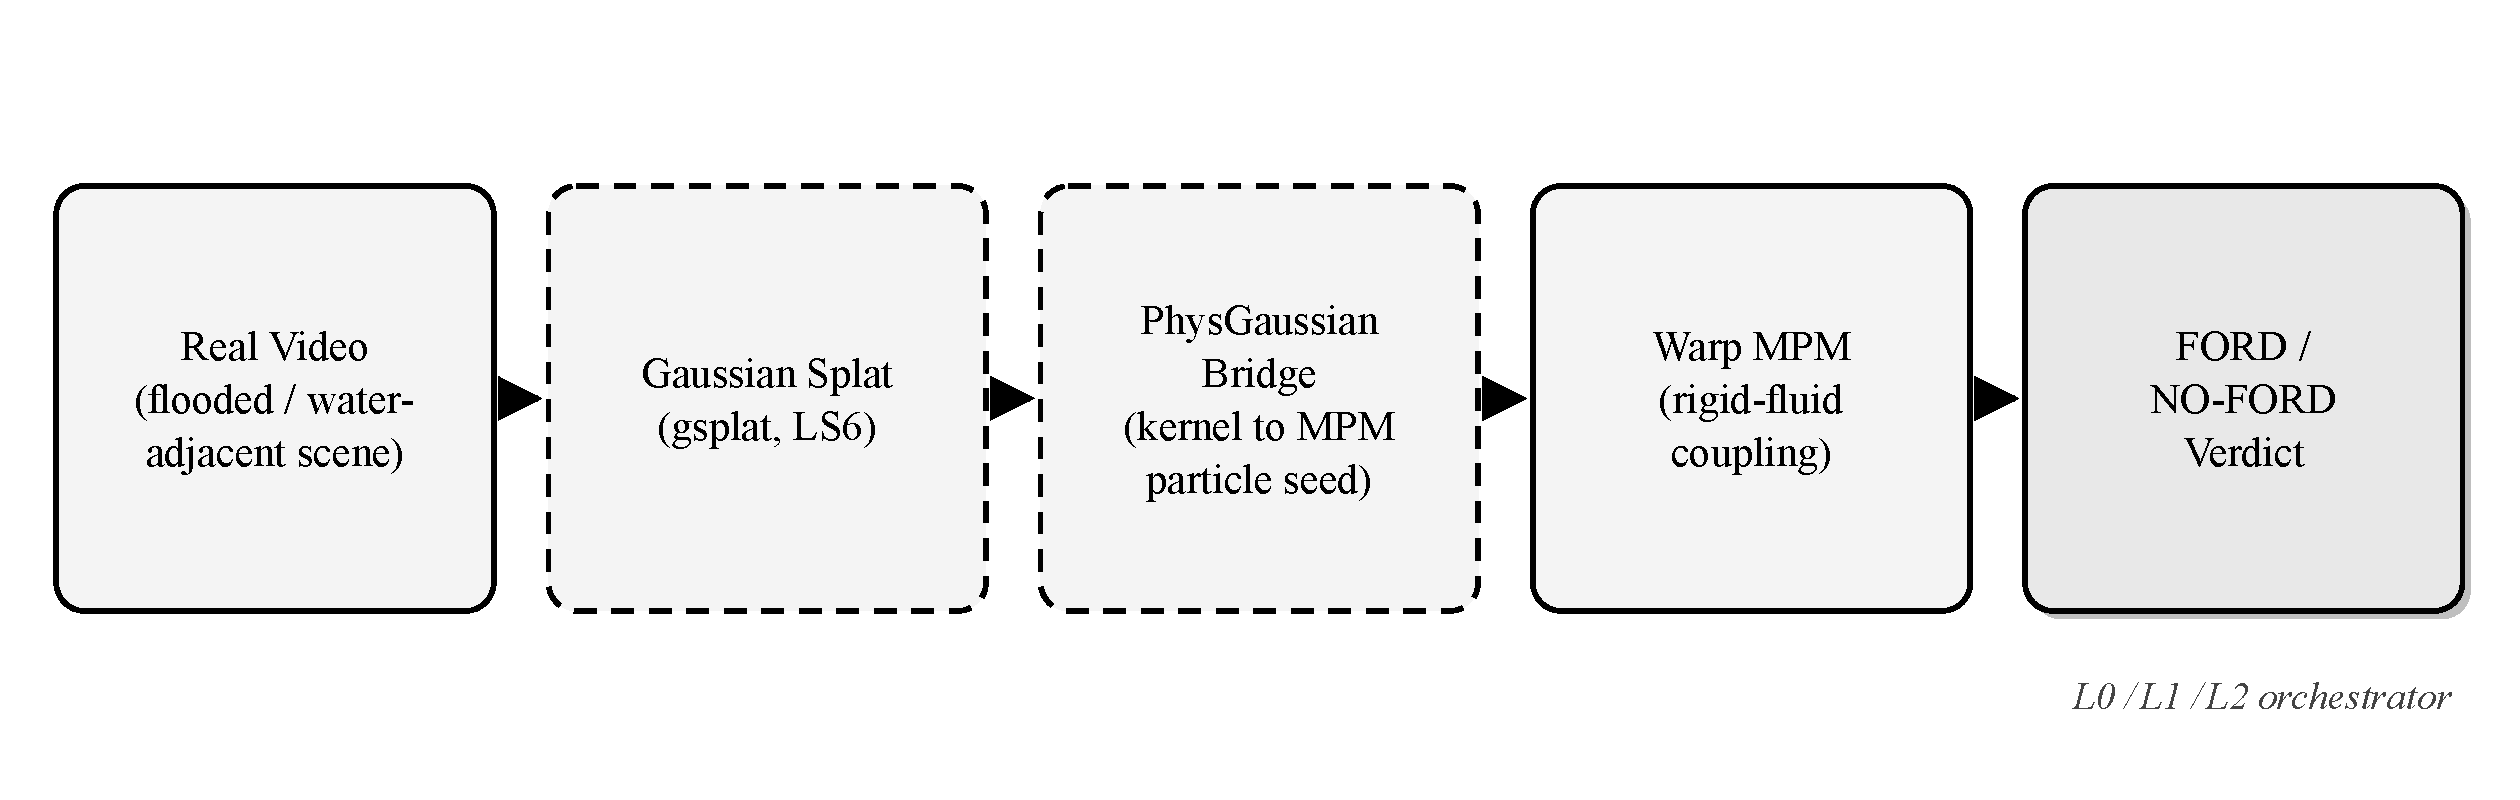
\includegraphics[width=0.92\textwidth]{figures_review/pipeline_diagram_v2.pdf}
\caption{The intended reconstruct-to-decide architecture: a real video would be reconstructed as a Gaussian splat, bridged to Material Point Method particles following PhysGaussian, simulated in Genesis with rigid-fluid coupling, and resolved to a FORD/NO-FORD verdict by the L0/L1/L2 abstraction orchestrator. This is a target design, and the stages are not equally realized. Dashed stages are conceptual, not the path used for any result reported here. The coupled MPM simulation and the verdict orchestrator are implemented and exercised throughout Section~\ref{sec:results}, but they are seeded from a watertight vehicle mesh rather than from a splat. The Gaussian-splat reconstruction and the PhysGaussian kernel-to-particle bridge are designed and not yet built: no trained splat has entered a simulation in this work, and the bridge does not exist as code. Readers should not infer that the chain has been executed end to end.}
\label{fig:pipeline}
\end{figure*}

% =================================================================
% II. PRIOR WORK
% =================================================================
\section{Prior Work}
\label{sec:prior}

\subsection{Flood-Vehicle Stability Criteria}
Two families of empirical criteria describe when floodwater destabilizes a vehicle. The Australian Rainfall and Runoff (AR\&R) Project 10 guidelines define a depth-velocity hazard scalar, $H = D \times V$ (m\textsuperscript{2}/s), with published class-specific thresholds \cite{shand2011}. Smith, Modra, and Felder report full-scale flotation and sliding stability curves derived from physical vehicle testing \cite{smithmodrafelder2019}. Both are single-number criteria: neither represents the direction of applied force, and neither was derived to predict the persistent lateral drift this project observes at some phase-space points (Section~\ref{sec:results}).

\subsection{Physics-Grounded Scene Reconstruction}
3D Gaussian Splatting (3DGS) reconstructs a photorealistic, explicit scene representation from ordinary multi-view video \cite{kerbl20233dgs}. PhysGaussian extends this representation with physical simulation by treating each Gaussian kernel's covariance as a seed for a continuum Material Point Method (MPM) particle volume, allowing a trained splat to drive a physics simulation directly rather than only a renderer \cite{xie2023physgaussian}. The simulation itself runs in Genesis, an open-source, solver-agnostic physics engine \cite{genesis2024}. No publicly available, drop-in flood-video-to-Genesis-MPM pipeline exists as of this writing; PhysGaussian's own reference implementation targets a Warp MPM solver, not Genesis.

\subsection{Why a Single Scalar Threshold Is Insufficient}
Both L0 and L1 are deterministic functions of published thresholds, not simulation output: L0 applies a single fixed depth cutoff \cite{nws_tadd}, and L1 applies the AR\&R two-part depth-and-hazard criterion per vehicle class \cite{shand2011}. We evaluate both across the same depth-velocity grid. Fig.~\ref{fig:l0l1} shows that L0 alone is markedly over-conservative, and that AR\&R's own published per-class caps (Fig.~\ref{fig:threeclass}) already diverge well before any coupled simulation is involved. Neither figure required simulated data; both are direct evaluations of cited formulas, and both motivate why a coupled physical model is worth the added cost.

\begin{figure*}[t]
\centering

\includegraphics[width=\linewidth]{figures_review/l0l1_two_rules_v2.pdf}
\caption{L0 (fixed depth threshold) versus L1 (AR\&R depth-velocity criterion) across all 70 (depth, velocity) scenarios of \texttt{data/scenario\_sweep.csv}. Both panels are direct evaluations of published formulas \cite{nws_tadd,shand2011}, not simulation output, and both read their verdicts from stored columns rather than recomputing a threshold. Left: the \emph{bare} rule (\texttt{L1\_haz\_product\_only}), which tests only $D \times V \le 0.60$\,m\textsuperscript{2}/s and permits crossing in 37 of 70 scenarios, 30 of them where L0 alone would refuse. Right: the \emph{joint} rule (\texttt{L1\_verdict}), which requires the class depth cap \emph{and} the $D \times V$ cap to hold together, permitting 14 of 70, only 7 of them beyond L0. The joint rule is canonical for this paper going forward; the bare rule is shown because it is the form in which the criterion is most often applied. The two panels differ in both rule structure and vehicle class: the left applies AR\&R's Large 4WD hazard cap alone ($D \times V \le 0.60$\,m\textsuperscript{2}/s, no depth restriction), the right the Small Car joint rule ($D \times V \le 0.30$\,m\textsuperscript{2}/s \emph{and} depth $\le 0.30$\,m); \texttt{L1\_verdict} is identical to \texttt{L1\_verdict\_small\_passenger} on all 70 rows. Of the 23 scenarios that reclassify from FORD to NO-FORD between the panels, 5 are excluded by the tighter hazard cap alone, 10 by the depth cap alone, and 8 by both, and none reclassify in the opposite direction. The depth cap is not redundant with the hazard cap: 7 of the 23 are standing water at zero velocity and depths of 0.40 to 1.00\,m, which a product-only threshold permits at any depth because $D \times V = 0$.}
\label{fig:l0l1}
\end{figure*}

\begin{figure}[t]
\centering
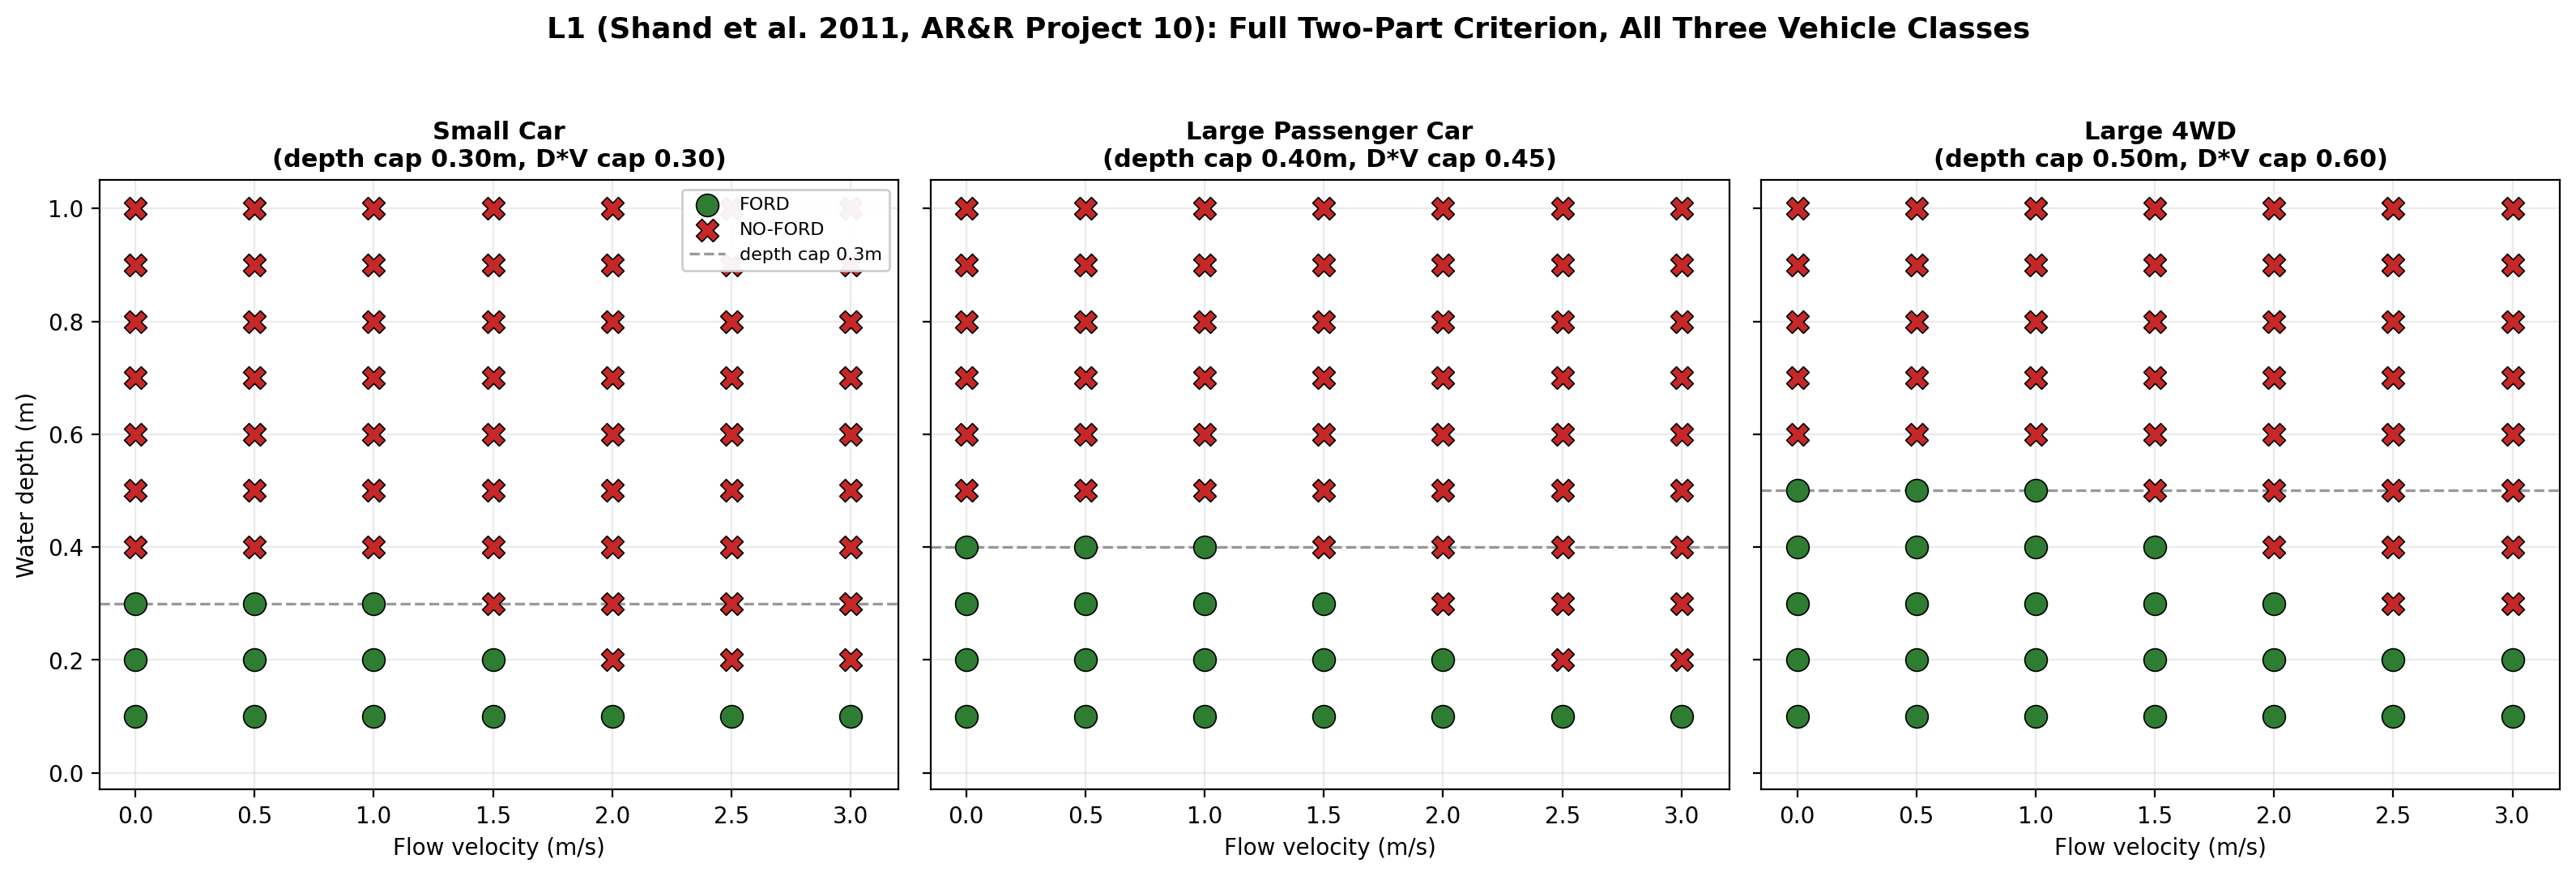
\includegraphics[width=\linewidth]{../figures/L1_three_class_corrected.png}
\caption{The L1 criterion evaluated under AR\&R's full two-part rule (depth cap \emph{and} $D \times V$ cap) for each of AR\&R's own three published vehicle classes \cite{shand2011}: Small Car (0.30\,m, 0.30\,m\textsuperscript{2}/s), Large Passenger Car (0.40\,m, 0.45\,m\textsuperscript{2}/s), and Large 4WD (0.50\,m, 0.60\,m\textsuperscript{2}/s). Panels correspond to the \texttt{L1\_verdict\_small\_passenger}, \texttt{L1\_verdict\_large\_passenger}, and \texttt{L1\_verdict\_large\_4wd} columns of \texttt{data/scenario\_sweep.csv}, which permit crossing in 14, 19, and 26 of the 70 scenarios respectively; the three classes disagree on 12 of the 70. These are AR\&R's own vehicle-weight categories, defined by mass and stability class in the source guideline, and are not a body-style mapping onto the sedan/SUV/pickup NHTSA/SAE classes of Table~\ref{tab:vehicle}; the two taxonomies are independent and should not be read as the same three vehicles.}
\label{fig:threeclass}
\end{figure}

\subsection{Forward and Inverse Property Estimation}
Hsiao and Kumar demonstrate the inverse direction of this same reconstruction-to-physics pipeline: given only visual observation, a NeRF-based reconstruction paired with Bayesian optimization recovers a granular material's friction angle to within roughly two degrees of ground truth \cite{hsiaokumar2025}. This project addresses the complementary forward direction: given a known scene and known flood hydraulic conditions, what is the traversability verdict under full fluid-rigid-body dynamics? Together, the two directions describe a closed perception-to-action loop, one of the auditability properties PVWM requires \cite{thorpe2026pvwm}.

% =================================================================
% III. APPROACH
% =================================================================
\section{Approach}
\label{sec:approach}

\subsection{Pipeline}
The reconstruct-to-decide pipeline (Fig.~\ref{fig:pipeline}) has four stages: (1) a real flooded or water-adjacent road scene is captured on video and reconstructed in 3D via Gaussian splatting on an NVIDIA A100 GPU (TACC Lonestar6); (2) following the PhysGaussian extraction pattern, trained Gaussian kernels are opacity-filtered and converted into an initial MPM particle volume; (3) the particle volume, together with a rigid-body vehicle proxy, is simulated in the Genesis physics engine using weakly-compressible MPM water and rigid-MPM coupling; (4) the simulation's displacement output is passed through a query-conditioned abstraction-selection orchestrator, \texttt{orchestrate\_ford\_query()}, which returns a FORD/NO-FORD verdict at the cheapest level of fidelity sufficient to answer correctly.

\subsection{Three-Level Abstraction Ladder}
We compare three levels of physical fidelity on the same phase-space grid of (depth, velocity) conditions, summarized in Table~\ref{tab:ladder}.

\begin{table}[t]
\caption{Abstraction Ladder Definitions}
\label{tab:ladder}
\centering
\begin{tabular}{@{}p{0.3in}p{0.85in}p{1.95in}@{}}
\toprule
\textbf{Level} & \textbf{Basis} & \textbf{Definition} \\
\midrule
L0 & Static depth & Fixed depth cutoff ($\approx$0.15\,m \cite{nws_tadd}), independent of velocity or vehicle class. \\
L1 & Depth-velocity scalar & $H = D \times V$ vs.\ an AR\&R per-class threshold \cite{shand2011}; the class is stated wherever L1 is evaluated rather than fixed globally. Section~\ref{sec:prior} uses the Large 4WD cap (0.60\,m\textsuperscript{2}/s), the least restrictive of the three, to show that L0 is over-conservative even against the most permissive published class. Section~\ref{sec:results} instead uses the Small Car cap (0.30\,m\textsuperscript{2}/s), which is the class matching the 1100\,kg curb weight of the hull actually simulated, and is therefore the more physically defensible choice for that experiment. $V$ is flow velocity, not vehicle speed; mass and force direction are not represented. \\
L2 & Coupled MPM & Genesis rigid-MPM simulation; NO-FORD when lateral drift exceeds a threshold. The threshold is 0.05\,m, an internally-chosen, uncited, conservative onset-of-motion detection value, not a literature stability criterion. \\
\bottomrule
\end{tabular}
\end{table}

This instantiates the orchestrator PVWM leaves unimplemented: the empirical L1/L2 divergence zone characterized in Section~\ref{sec:results} defines the escalation boundary at which L1 alone is not sufficient and the query must be answered at L2.

A first-principles force balance motivates why L1's scalar hazard measure is expected to be insufficient. Fig.~\ref{fig:force} plots lateral hydrodynamic drag force against maximum available static friction, using the tire-road friction coefficient range reported for flood conditions by Azhar et al.\ \cite{azhar2023}, at several water depths (left), and the resulting critical velocity above which drag is predicted to exceed friction, as a function of depth (right). The friction coefficient implied by that figure is $\mu = 0.350$, inside the range Azhar et al.\ report \cite{azhar2023}. \FLAG{Still open: the drag coefficient and frontal area behind this figure have not been traced to a cited source, and no generating script for it exists in the repository, so the drag equation itself cannot yet be quoted. Either recover or rewrite the generator before submission, or state the drag formulation explicitly in the caption.}

\begin{figure}[t]
\centering
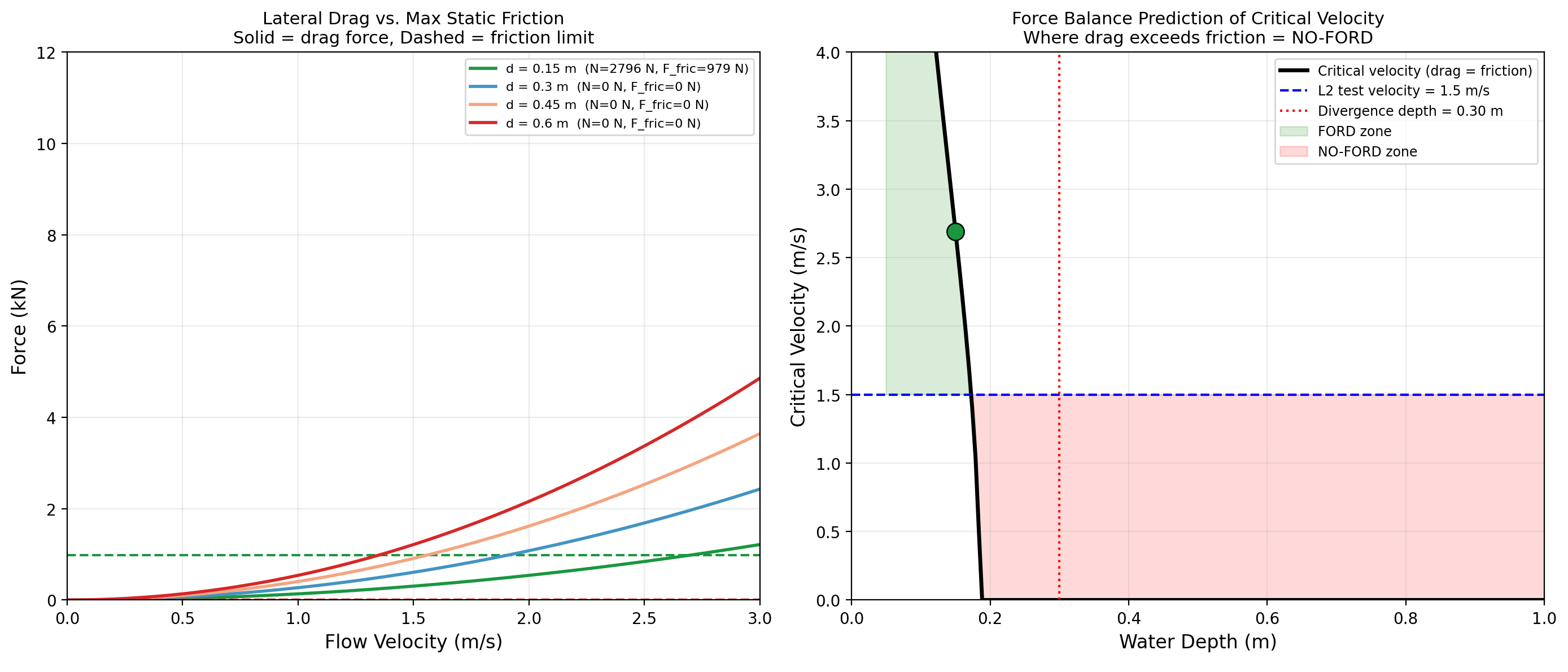
\includegraphics[width=\linewidth]{force_balance.png}
\caption{Analytical force-balance calculation, not simulation output. Left: lateral drag force versus flow velocity at four water depths, against the maximum static friction limit (dashed). Right: the resulting critical velocity, above which drag exceeds friction, as a function of depth. The legend reports $N=0$ and $F_{\text{fric}}=0$ at 0.30, 0.45, and 0.60\,m. Those zeros are a real buoyancy result, not missing values: at 0.30\,m this model's buoyant force already reaches 15.99\,kN against a vehicle weight of 10.79\,kN, so normal force is zero and the friction limit $\mu N$ vanishes with it. The right panel corroborates this independently, with critical velocity falling to zero near 0.19\,m. That flotation depth is a property of the model's displacement assumption, which treats the vehicle as a solid prism over roughly three quarters of its bounding-box footprint. The real hull encloses 3.5427\,m\textsuperscript{3} against a 10.7457\,m\textsuperscript{3} bounding-box prism, a fill factor of only 0.33, so the prism assumption overstates displacement in shallow water and floats the vehicle at about 0.20\,m. That is below even the 0.30\,m depth cap AR\&R assigns to its Small Car class \cite{shand2011}, so the model reaches flotation before the empirical guideline reaches its own depth limit. This figure should therefore be read as establishing the \emph{shape} of the drag-versus-friction argument, not as a calibrated flotation prediction. \FLAG{Project notes record a measured critical flow depth of about 0.38\,m for a full-scale passenger vehicle, which would sharpen this comparison, but the corresponding bibliography entry is an unverified placeholder and is deliberately not cited here. Verify that reference before quoting the 0.38\,m figure in the paper.}}
\label{fig:force}
\end{figure}

\subsection{Vehicle and Scene Representation}
The vehicle is a single watertight triangle mesh derived from the CCSA/GMU coarse 2010 Toyota Yaris crash-test finite-element deck \cite{ccsa2010yaris}, a 378{,}376-element model whose own header gives a curb mass of 1100\,kg. That deck is not simulation-ready as distributed: it is an assembly of 919 shell, solid, and beam parts that interleaves exterior body panels with zero-thickness interior trim, not a closed surface. Conversion therefore proceeds in two stages. First, the \texttt{*NODE}, \texttt{*ELEMENT\_SHELL}, and \texttt{*ELEMENT\_SOLID} cards are read directly by fixed-width manual parsing and filtered to exterior-body parts, bypassing the compiled deck reader, which stalls on this file and whose summary output reports keyword-section counts rather than element counts. Second, the extracted surface is voxel-remeshed into a closed manifold with \texttt{mesh2sdf}. We chose voxel remeshing over surface-topology hole filling because, given the mixed interior and exterior parts, direct hole filling risks sealing the underbody shut and silently corrupting the enclosed volume on which the buoyancy term depends. The resulting hull has 327{,}212 vertices, 655{,}308 faces, and an enclosed volume of 3.542739\,m\textsuperscript{3}. All 17 gated coupled runs reported in Section~\ref{sec:results} use this one mesh; no box proxy and no rescaled silhouette enters the L2 results.

The three AR\&R stability classes are realized as \emph{mass overrides applied to that same hull}, not as three distinct vehicle geometries. The sweep driver assigns 1100, 1609, and 2337\,kg to the identical mesh and re-solves, so the solid particle count is unchanged across the three runs at a given grid resolution. Cross-class comparison in this paper therefore isolates the effect of mass alone, with footprint, hull volume, and inertia tensor held fixed. This is a deliberate scope choice and also a limitation: it cannot speak to how body shape affects traversability, only how mass does.

Two consequences follow, and they should not be conflated. First, particle density is not a material constant in these runs; it emerges per run as mass divided by realized solid volume, and therefore varies with both the assigned mass and the grid resolution, as summarized in Table~\ref{tab:vehicle}. Second, the three passenger-vehicle classes defined in the project's own \texttt{vehicle\_params.py} (1100, 1990, and 2300\,kg, with per-class bounding boxes from NHTSA/SAE reference data \cite{sae1999011336}) are a separate parameter system that was \emph{not} used for the coupled runs; the AR\&R masses above come from the stability guideline's class definitions instead. The two systems share only the 1100\,kg entry and should not be read as the same three classes.

\begin{table}[t]
\caption{Realized Particle Density per Coupled Run, One Hull, Three AR\&R Mass Overrides}
\label{tab:vehicle}
\centering
\begin{tabular}{@{}p{0.62in}p{0.42in}p{0.62in}p{0.72in}@{}}
\toprule
\textbf{AR\&R class} & \textbf{Mass (kg)} & \textbf{$n_{\text{grid}}$} & \textbf{Realized $\rho$ (kg/m\textsuperscript{3})} \\
\midrule
Small Car      & 1100 & 48 / 64 / 96 & 302.6 / 309.7 / 312.3 \\
Large Pass.\   & 1609 & 48 / 64 / 96 & 442.6 / 453.1 / 456.9 \\
Large 4WD      & 2337 & 48 / 64 / 96 & 642.8 / 658.1 / 663.6 \\
\bottomrule
\end{tabular}
\\[2pt]
{\footnotesize All nine rows share one hull of volume 3.542739\,m\textsuperscript{3}. Density is computed at run time as mass divided by realized solid particle volume, not assigned; it therefore rises slightly and monotonically with grid resolution even at fixed mass, as finer voxelization fills the hull more completely. Values above 300\,kg/m\textsuperscript{3} exceed the 100--300\,kg/m\textsuperscript{3} effective-density band used as an early sanity heuristic in this project; that band was calibrated against a hollow box proxy and does not apply to a solid-filled watertight hull, so it is reported here rather than treated as a failed check.}
\end{table}

% =================================================================
% IV. RESULTS
% =================================================================
\section{Results}
\label{sec:results}

\subsection{Scene Reconstruction Status}
Structure-from-motion reconstruction (COLMAP) is complete for one real scene (``Drain A''), confirmed via a populated sparse point cloud and camera pose set on TACC Vista scratch storage. \FLAG{Gaussian-splat checkpoint training from this reconstruction, which runs separately on LS6, has not been confirmed complete as of this draft. Do not describe Drain A as a fully trained, simulation-ready splat until that is verified live. A second scene (``Drain B'') has not yet been captured or reconstructed.}

\subsection{Synthetic-Geometry Pilot Study}
A synthetic-geometry pilot compared the L1 criterion against the coupled L2 solver at nine (depth, velocity) conditions, shown in Fig.~\ref{fig:l2schematic}. The two rungs agree at five of the nine conditions and disagree at four, an agreement rate of 55.6\%. Every disagreement runs in the same direction: L1 permits crossing where L2 refuses it, and there is no condition in this dataset where L1 is the more conservative rung. All four divergent conditions lie inside the L1 iso-hazard boundary, that is, in the region a scalar $D \times V$ test alone would clear. They cluster at shallow-to-moderate depth (0.15--0.30\,m) with sustained flow (1.0--2.0\,m/s), which is the regime where the scalar measure has no mechanism to represent directional, persistent lateral force.

Two scope limits belong with these numbers. First, the L1 verdicts in this pilot are the \emph{bare} product rule at a 0.60\,m\textsuperscript{2}/s cap, taken from the dataset's own stored threshold, not the class-specific joint rule that Fig.~\ref{fig:threeclass} and the rest of Section~\ref{sec:results} use; the two are different criteria and the 55.6\% figure is specific to the bare form. Second, nine conditions is a pilot, not a converged sampling of the phase space, and the geometry was synthetic rather than the reconstructed scene. \FLAG{Still open, narrowed: at (0.30\,m, 1.5\,m/s) the source dataset's \texttt{l1\_haz\_score} field records 0.750 where $D \times V$ is 0.450. The plotted and quoted values use \texttt{dv\_product}, which is self-consistent and agrees with that row's stored verdict, but the corrupt cell should be traced or corrected at source before the dataset is published.}

\begin{figure}[t]
\centering
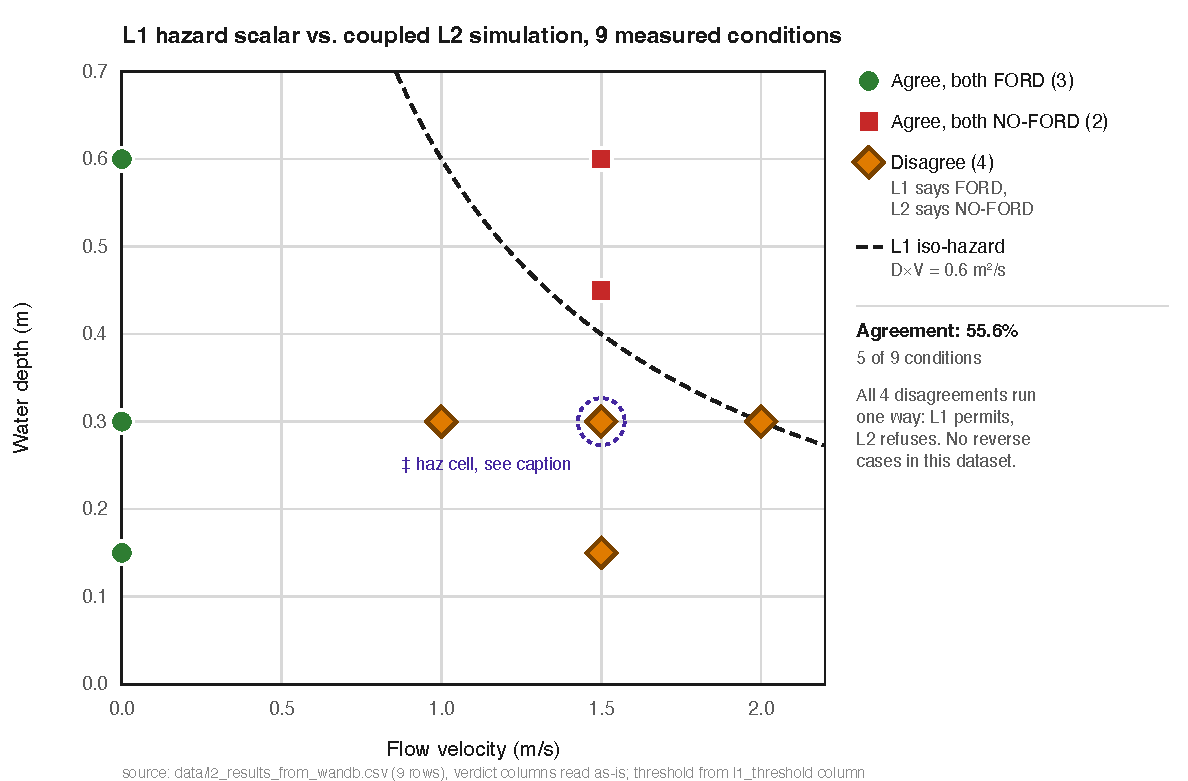
\includegraphics[width=\linewidth]{figures_review/l2_divergence_real_v2.pdf}
\caption{Measured L1-versus-L2 agreement at the nine (depth, velocity) conditions of the synthetic-geometry pilot, from \texttt{data/l2\_results\_from\_wandb.csv}. Three conditions permit crossing at both rungs, two refuse at both, and four disagree, giving 55.6\% agreement. Every disagreement is L1-permissive and L2-restrictive; there are no reverse cases. The dashed curve is the L1 iso-hazard boundary $D \times V = 0.60$\,m\textsuperscript{2}/s, read from the dataset's own threshold field, and all four divergent conditions fall inside it. L1 verdicts here are the bare product rule, not the class-specific joint rule of Fig.~\ref{fig:threeclass}. $\ddagger$ marks the one condition whose stored hazard field disagrees with $D \times V$; the plotted value is $D \times V$ (see body text).}
\label{fig:l2schematic}
\end{figure}

\subsection{Real-Simulation Sweep}
\label{subsec:sweep}
The coupled sweep reported here is the gated run inventory in \texttt{data/all\_runs\_inventory.csv}: 17 runs on the watertight Yaris hull, all under a standing-water-plus-sustained-inflow scenario at a floor friction of 0.55. It comprises a 3\,$\times$\,3 mass-by-resolution block at fixed depth 0.30\,m and velocity 1.5\,m/s, a three-point depth sweep, and a five-point velocity sweep. An earlier 36-run sweep (referred to in project notes as ``v2'') is \emph{not} cited here and is not a source for any figure in this paper: it was run on a rescaled box proxy of 1390\,kg enclosing 4.7352\,m\textsuperscript{3}, against the real hull's 3.5427\,m\textsuperscript{3}, and is superseded by the runs above.

Fig.~\ref{fig:masssweep} shows the mass-by-resolution block. Displacement falls monotonically as mass rises at every one of the three grid resolutions tested, so the \emph{direction} of the mass effect is consistent. The \emph{magnitude} is not: the three curves do not overlay, and the 48- and 64-cell curves cross between 1609 and 2337\,kg. The lightest-to-heaviest displacement ratio is non-monotonic in resolution across the three grids, so no single multiplier characterizes the mass effect and none is quoted here. Any mass-sensitivity claim from this work is therefore directional only, and treating it as a calibrated effect size would be unsupported.

Two honesty constraints travel with this dataset. First, particle passthrough exceeds the project's 10\% acceptance limit in 7 of the 17 runs, concentrated at the lightest mass and at the highest velocities, reaching 15.9\% at 3.0\,m/s. Those runs are flagged in Fig.~\ref{fig:masssweep} rather than dropped, since removing them would silently bias the sweep toward its better-resolved corner. Second, water-layer depth resolution varies across the block, from three layers at the coarsest grid to six at the finest, so the coarse-grid rows are the least trustworthy independent of their passthrough figure. \FLAG{Still open: the L2 verdict threshold remains 0.05\,m of lateral drift with no independent citation, so verdict counts from this sweep are deliberately not reported here; only the continuous displacement measure is. Resolve the threshold provenance before converting this sweep into FORD/NO-FORD counts.}

\begin{figure}[t]
\centering
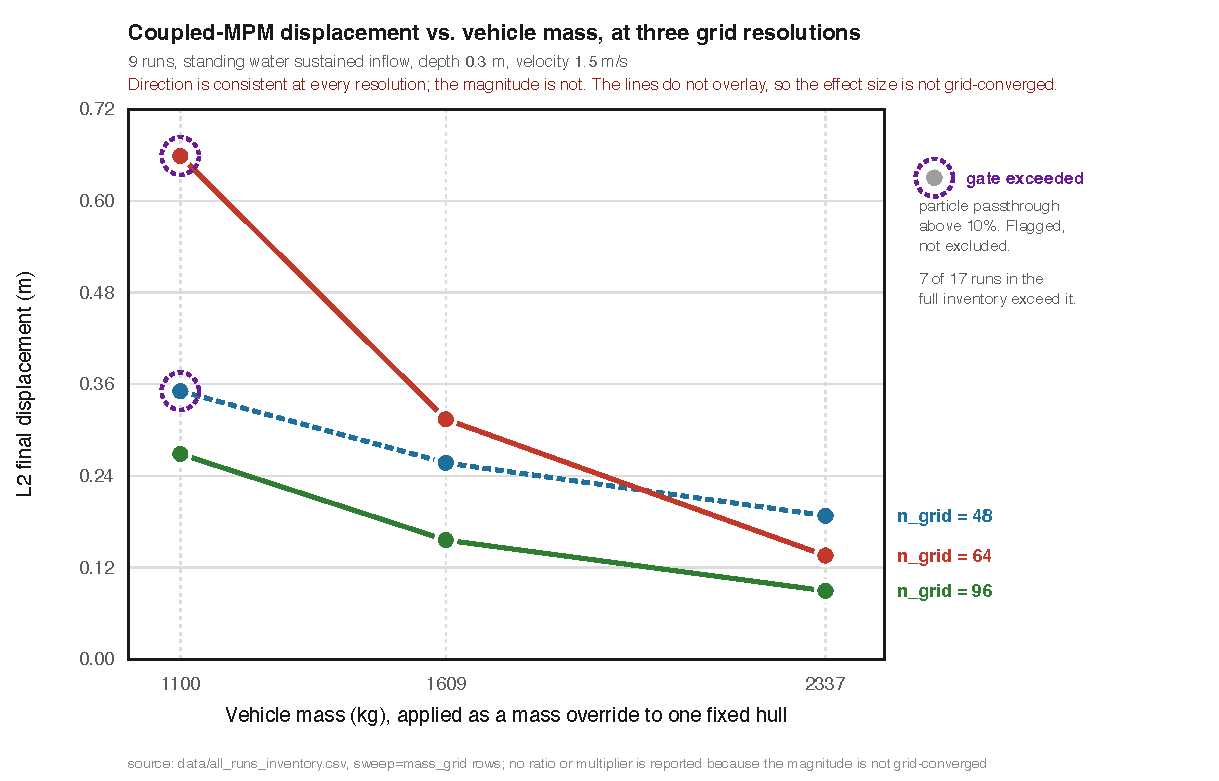
\includegraphics[width=\linewidth]{figures_review/mass_grid_sweep_v2.pdf}
\caption{The direct visual for the 3\,$\times$\,3 mass-by-resolution block described in Section~\ref{subsec:sweep}: coupled-MPM final displacement versus vehicle mass at three grid resolutions, from the nine \texttt{sweep=mass\_grid} rows of \texttt{data/all\_runs\_inventory.csv}. One hull, three AR\&R mass overrides, fixed depth 0.30\,m and velocity 1.5\,m/s. Displacement decreases with mass at every resolution, but the curves do not collapse onto one another and the 48- and 64-cell curves cross, so the effect size is not grid-converged; no ratio or multiplier is reported for this reason. Ringed markers exceed the 10\% particle-passthrough limit and are flagged rather than excluded; 7 of the 17 runs in the full inventory exceed it.}
\label{fig:masssweep}
\end{figure}

% =================================================================
% V. CONCLUSIONS
% =================================================================
\section{Conclusions}
\label{sec:conclusions}

The synthetic-geometry pilot demonstrates, as a proof of concept, that a scalar depth-velocity hazard measure can disagree substantially with a coupled physical simulation, and that the disagreement is structural rather than a calibration artifact: no choice of coupling friction closes the gap at the divergence points identified in Section~\ref{sec:results}. This supports treating abstraction selection as query-dependent rather than assuming any single fixed-fidelity model is correct everywhere in the operating envelope. \FLAG{This is the pilot-study conclusion. Do not upgrade this to a claim about the real reconstructed scene until the real-scene sweep in Section~\ref{sec:results} is verified and the vehicle mesh/density limitation is either resolved further or explicitly scoped as a stated limitation.}

% =================================================================
% VI. FUTURE WORK
% =================================================================
\section{Future Work}
\label{sec:future}

We identified several concrete extensions, listed roughly in order of expected impact relative to effort.

\begin{itemize}
\item \textbf{Distinct geometry per vehicle class.} The crash-validated NCAC 2010 Toyota Yaris hull is already in use here (Section~\ref{sec:approach}), so the remaining gap is not obtaining one validated mesh but obtaining several. The three classes in this paper differ only by assigned mass on that single hull. Converting a second and third NCAC model, such as the 2007 Chevrolet Silverado pickup, from LS-DYNA keyword format to watertight collision meshes would let body shape and footprint vary alongside mass, which is the one axis the present cross-class comparison cannot address.
\item \textbf{Physical-viability audit dashboard.} A direct instantiation of PVWM's ``physically viable'' criterion: automated checks for mass conservation, momentum conservation, MPM Jacobian/volume-ratio bounds, zero-penetration contact, and energy monotonicity, applied to every run rather than asserted informally.
\item \textbf{Failure-mode classification with violation magnitude.} An explicit failure-mode hierarchy (stuck, slide, topple, float) reported with the magnitude by which a run crosses each threshold, rather than a binary verdict.
\item \textbf{Graph Network Simulator (GNS) surrogate.} A lightweight GNS trained on the completed simulation sweep as a fast surrogate for untested (depth, velocity, vehicle-class) combinations, connecting the L0/L1/L2 ladder to a learned, still physically-grounded fourth level.
\item \textbf{A second independently-sourced real scene.} \FLAG{Verify exact citation and public availability of the FRED flooded-road dataset before including it as a committed future-work item rather than a candidate.}
\item \textbf{DesignSafe-CI dataset publication.} Publish the validated real-scene dataset and simulation outputs with a DOI once the real-scene sweep is verified, rather than publishing the synthetic pilot data.
\end{itemize}

% =================================================================
% ACKNOWLEDGMENT
% =================================================================
\section*{Acknowledgment}
This work was supported by the National Science Foundation under NSF REU Site: Cyberinfrastructure Research for Societal Advancement (SCIPE-AI), Award \#2447887, hosted at the Texas Advanced Computing Center (TACC), The University of Texas at Austin. The author thanks faculty mentor Dr.\ Krishna Kumar and research mentors Hassan Iqbal, Cheng-Hsi Hsiao, and Cristian Moran for their guidance throughout this project, and Rosalia Gomez for program coordination and support.

% =================================================================
% REFERENCES
% Uses BibTeX + IEEEtran.bst, matching the Zotero/Better-BibTeX
% auto-export pipeline. The official Overleaf gallery IEEE template
% does not ship IEEEtran.bst by default; upload the one provided
% alongside this file, or references will not resolve.
% =================================================================
\bibliographystyle{IEEEtran}
\bibliography{can_it_ford_references_IEEE}

\end{document}
